\newif\ifdraft
\ifx\dontdraft\relax
\message{IFX TRUE}
\draftfalse
\else
\message{IFX FALSE}
\drafttrue
\fi

\documentstyle[a4,isolatin1,times, concmath, ht01e, graphicx]{article}

\ifdraft
\renewcommand{\baselinestretch}{0.9}
\def\margincomment#1{
\marginpar{
\vbox{
\scriptsize #1
}
}}
\def\nakki#1{\marginpar{\bf Nakki: #1}}
\pagestyle{plain}
\else
\def\margincomment#1{}
\def\nakki#1{}

% Make the times fonts defaults again if not draft.
\renewcommand{\sfdefault}{phv}
\renewcommand{\rmdefault}{ptm}
\renewcommand{\ttdefault}{pcr}

\fi


\newcommand{\url}[1]{\textsf{#1}}
\newcommand{\hyp}{\discretionary{}{}{}}

% Define a macro for your own margin notes here
% If it is ABSOLUTELY clear that something is a typo, go ahead
% and fix it. But don't make any major changes to the text itself
% yet. Also, only propose rearrangements in the margin: CVS doesn't
% work too well with rearrangements and edits done by several
% people. I will be the editor until wed or thu.
\def\kkw#1{\margincomment{kkw: #1}}

\def\ra{$\rightarrow$}

\ifdraft
\onecolumn
% \textwidth 8.5cm
\textwidth 9.6cm
\marginparwidth 8.5cm
\fi

\renewcommand\floatpagefraction{.9}
\renewcommand\topfraction{.9}
\renewcommand\bottomfraction{.9}
\renewcommand\textfraction{.1}   
\setcounter{totalnumber}{50}
\setcounter{topnumber}{50}
\setcounter{bottomnumber}{50}



\title{Awt (Associative writing tool): Supporting writing process with a ZigZag based writing tool -- work in progress}

\begin{document}

\def\figurewidth{\columnwidth}
\def\wfigurewidth{\textwidth}
\def\mockupwidth{16cm}

\ifdraft
\nocopyright
\fi

\authorname{Kimmo Wideroos
}
\authoraddr{  University of Jyv\"askyl\"a,
  Department of Mathematical Information Technology\\
  PO.~Box~35, FIN-40351~JYV\"ASKYL\"A, Finland\\
  E-Mail: kimmo.wideroos@cc.jyu.fi
}
\maketitle

\ifdraft
\begin{verbatim}
Id:.*
\end{verbatim}
\fi

\abstract
In this paper a sketch of a tool for supporting writing process is discussed 
as an example of an application using GZigZag framework.
GZigZag as well as Ted Nelson's ZigZag metastructure are introduced in 
a nutshell.

\paragraph{KEYWORDS:} supporting writing process, ZigZag metastructure, 
GZigZag, spatial hypertext, set based hypermedia 
\ifdraft
\vfill

\break
\tableofcontents

\vskip 0pt plus 2cm
\hrule
\vskip 0pt plus 2cm
\fi

%----------------------------------------------------------------------------
\section{INTRODUCTION: GZIGZAG}


GZigZag \cite{gzigzag} is a free \cite{GNU}
implementation of Ted Nelson's ZigZag design
\cite{zigzag-manual,zigzag-presentation,zigzag-welcome}.

In ZigZag, all data is represented as {\em cells} and connections
between cells along {\em dimensions}. 
Dimensions being orthogonal to each other makes it possible for one cell 
to be part in several substructures. 
In current implementation,
cells may contain references to extracts from permanent media scroll.
This feature guarantees unique identifiers for pieces of media 
({\em spans}) making referential Xanadu media model
\cite{literary-machines-931} possible in GZigZag. In practice
this means that copy\&paste operation, for example, causes an implicit link 
({\em transclusion}) between the contents, so that they can be easily detected and shown.  

\section{SUPPORTING WRITING PROCESS}
Traditional model of writing process is 
{\em prewriting \ra writing \ra rewriting}. Conventional wordprocessing 
programs support best this oversimplified (end product oriented) version of 
writing prosess. However, writing process has proved to be far more 
complicated than prewriting-writing-rewriting procedure can capture
\cite{hayes-flower86writing-research-and-the-writer}.

A fruitful way to consider writing is as an open-ended design task 
\cite{neuwirth89external-representations-in-writing},
where designers (writers) primary intention is not to make end product 
(linear document) but representations of it (externalize one's thoughts). 
Its is often reasonable to transfer the 
original design problem from actual domain to a more appropriate domain
({\em virtual world}) in order to bypass some constraints in the 'real' domain 
and make experiments easier \cite{schoen83reflection-in-on-action}.
Hypertext systems could provide this kind of virtual world for external
representations in cognitively complex tasks 
\cite{as-we-may-think, engelbart63conceptual-framework-augmenting-mans-intellect}
such as writing \cite{neuwirth89external-representations-in-writing}. 

Spatial hypertext widens conventional node-link hypertext model by 
taking advantage of spatial proximity and visual 
cues \cite{shipman-marshall00spatial-hypertext-alternative}, 
and is well suited to information intensive activities such as analysis, 
design and evaluation where domain 
structure is not well understood. ART (Amplifying Representational
Talkback) \cite{nakakoji00spatial-positioning} is an example of a tool 
that uses 2D spatial positioning enabling writer to externalize ideas in 
the early stages of writing. 

\section{ASSOCIATIVE WRITING TOOL}
The Awt (Associative writing tool) concept introduced here 
support spatial positioning of textual artefacts, organizing artefacts
in different sets (layers),
explicit links between artefacts and implicit Xanadu links between
contents of the artefacts. The implementation of Awt is currently 
work-in-progress; it will be included in gzigzag framework as a module in 
the near future. 

The entities of Awt information artefacts are derived from their 
connections in specific dimensions. Thus, a cell representing artefact 
can be interpreted as a set as well as an atomary information container 
depending on which dimensions are taken into consideration. The essential 
dimensions are the following (see also Fig. \ref{fig:view-zzstructure})
\begin{description}
\item[d.layerset] This connects set (or layer) cell and member cells via 
relation cells
\item[d.member] The last cell (positive end) in this rank is the member of
all sets connected via link cells in this rank 
\item[d.src] Headcell (negative end) of this rank is the source cell for
link cells connected along this rank
\item[d.trg] Positive end cell of this rank is the target of all link cells
along this rank
\end{description}

\begin{figure}[h]
\centering
\fbox{\includegraphics{view-zzstructure.epsi}}
\caption{Screenshots of two layer views and underlying zigzag-structure \
(only link and set related dimensions shown)}
\label{fig:view-zzstructure}
\end{figure}      

In Fig.\ref{fig:view-zzstructure} there is the ZigZag structure (or model)
shown below the dashed line. On the top there are two screenshots of views,
the left one has artefact A as layer artefact and the right one has C.

Notice the different roles of artefact C in the views (C is a note artefact 
in the right view, but a layer artefact in the left one having D as a member). 

Besides information of relations (link and set related), each artefact has 
spatial data as well as the content data stored in related substructures. 

\subsection{AWT AND SET BASED HYPERMEDIA}
In set based hypermedia model~\cite{parunak91set-based-hypermedia}, 
information nodes are not explicitly linked together as they are 
in graph-based hypermedia, but are implicitely related to eachother via 
sets, ie. by being members of the same set(s). According to Parunak 
\cite{parunak91set-based-hypermedia} set based hypermedia 
suits particularly well for taxonomic reasoning. Awt can be easily extended
to support set based hypermedia browsing operations, because it does
not require any changes in the underlaying zigzag model, 
(see Fig. \ref{fig:view-zzstructure}).
   
 

%\begin{itemize}

%	\item
%	story-telling vs. knowledge-transform
%	~\cite{bereiter87psychology-of-written-composition}

%	\item
%	normal vs. radical design
%	~\cite{vincenti92engineering-knowledge}

%	\item
%	reflection-in-action process
%	~\cite{nakakoji00spatial-positioning}

%	\item
%	spatial-hypertext
%	~\cite{}

%	\item
%	set-based-hypertext-taxonomic-reasoning
%	~\cite{}

%	\item
%	virtual-worlds
%	~\cite{}

%	\item
%	talkback in design
%	~\cite{nakakoji98representational-talkback-in-design}

%	\item
%	bottom-up vs. top-down
%	~\cite{sumi97computer-aided-thinking-and-metric-spaces}

%	\item
%	computer supported tools for writing: surface vs. logic and content
%	~\cite{carlson90nn-as-cogn-tools-for-writing}

%\end{itemize}

%\emph{Standards Track}\/ 

%\kkw{}

%\begin{figure}[htb!]
%\vbox{
%a) \\ 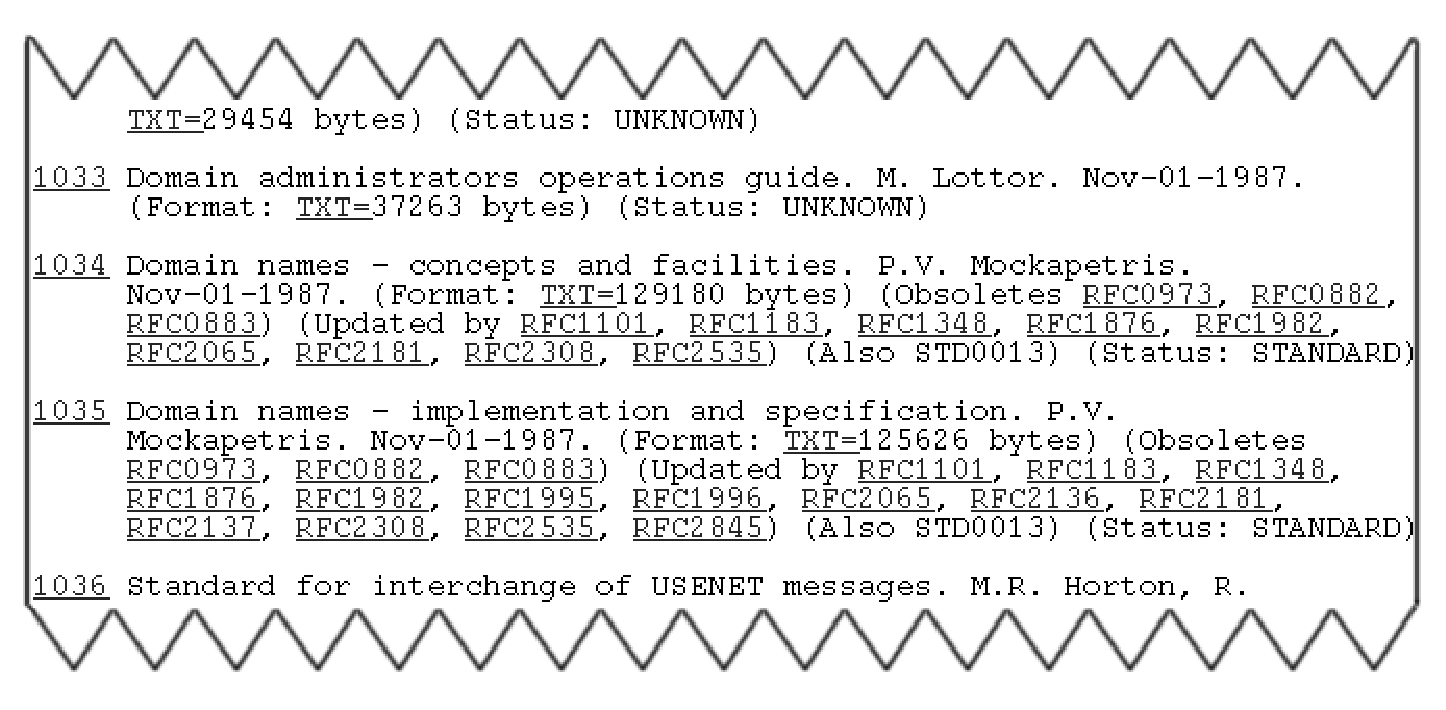
\includegraphics[width=\figurewidth]{HTML-RFC-index.ps} \\
%b) \\ 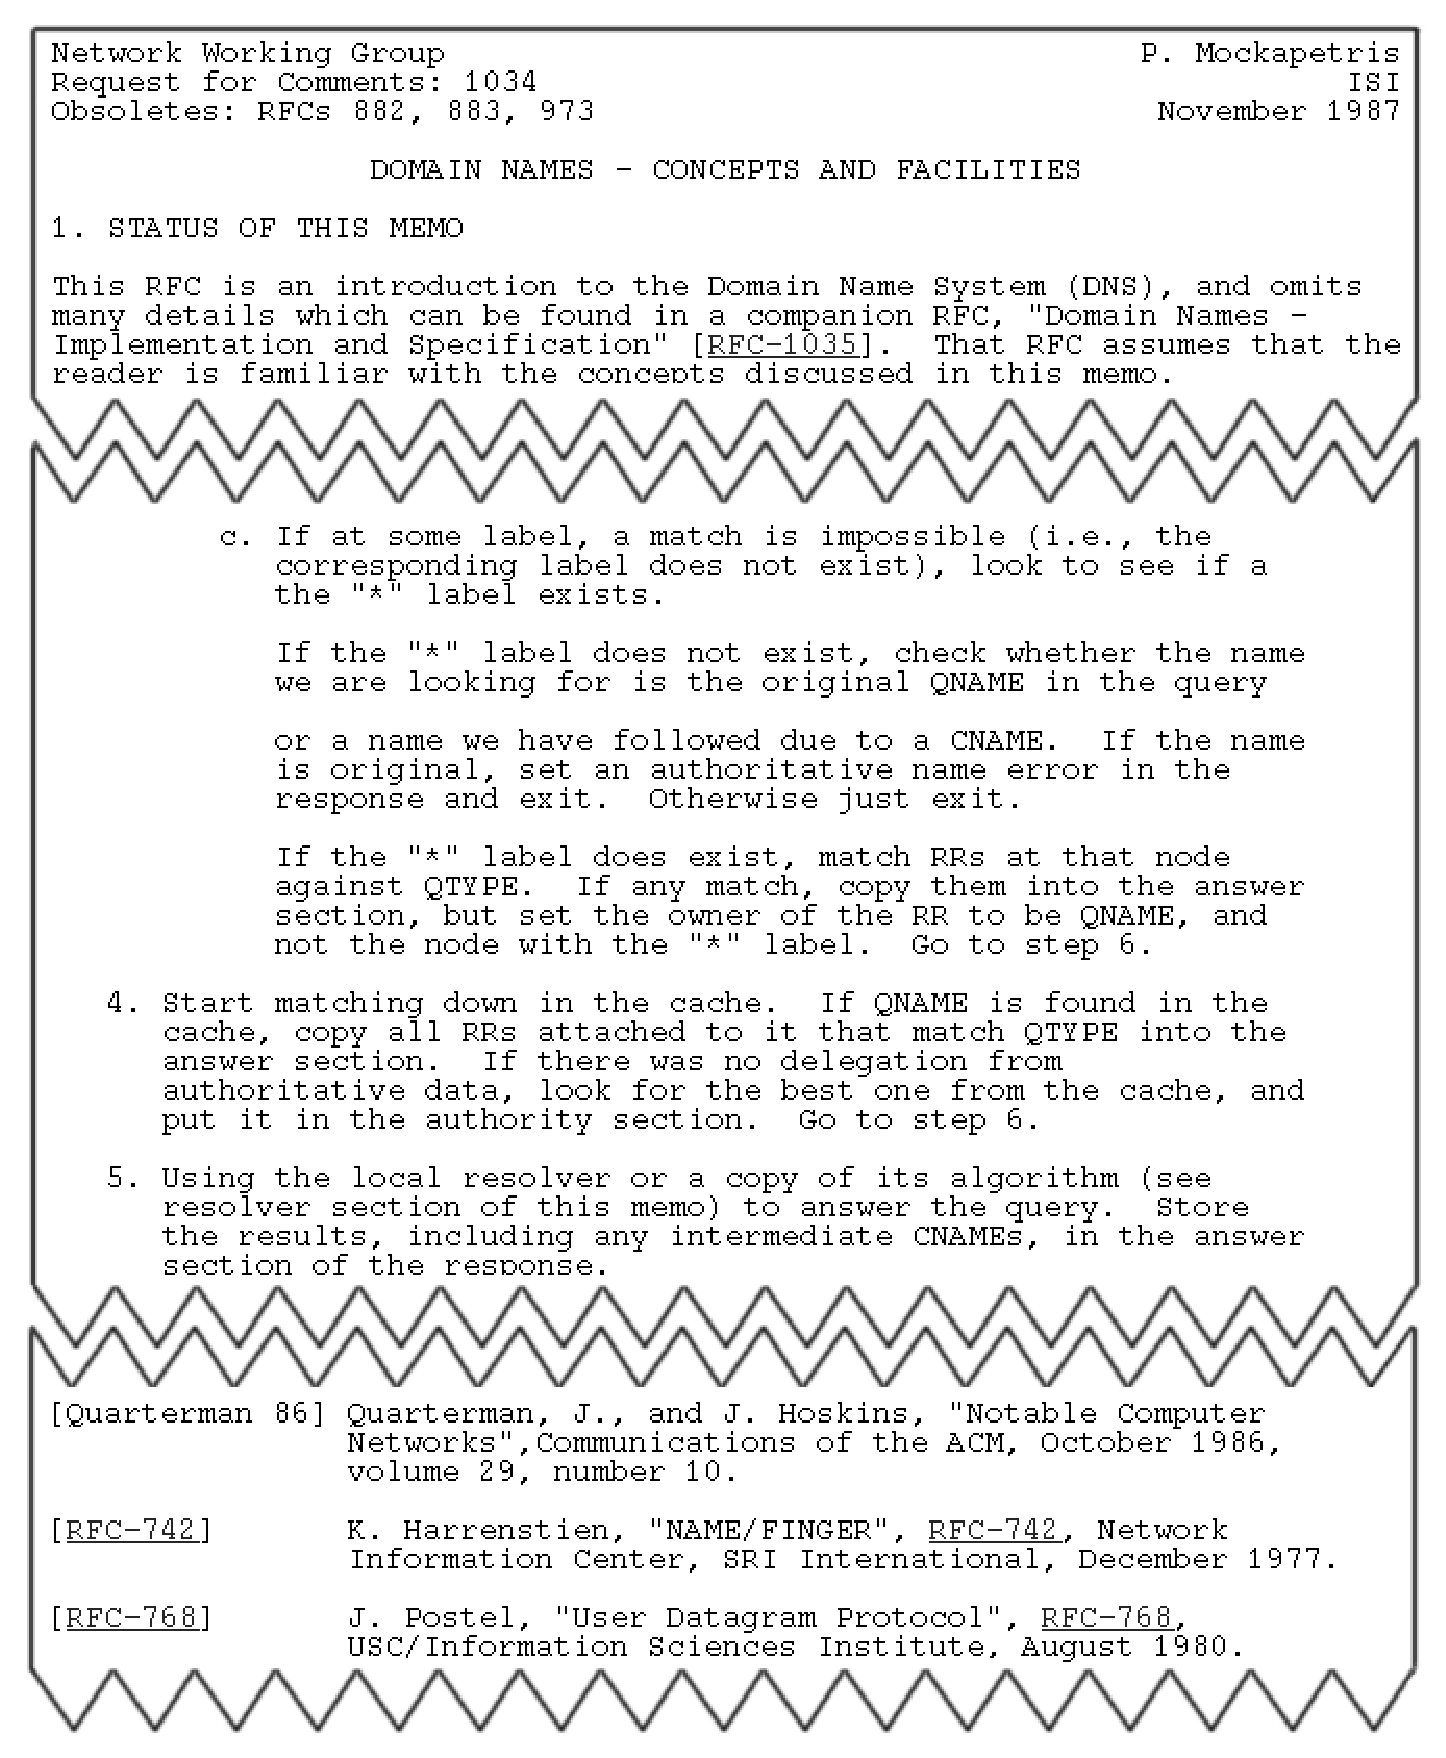
\includegraphics[width=\figurewidth]{HTML-RFC.ps}
%}
%\caption{a)The index entry at \cite{rfc-index-faqs} for RFC 1034
%b) Fragments of the HTML version of RFC 1034 from \cite{rfc-index-faqs}.
%\label{fig-example-current}}
%\end{figure}

%\ref{fig-example-current}

%\begin{figure*}[htb!]
%\centering
%\fbox{
%       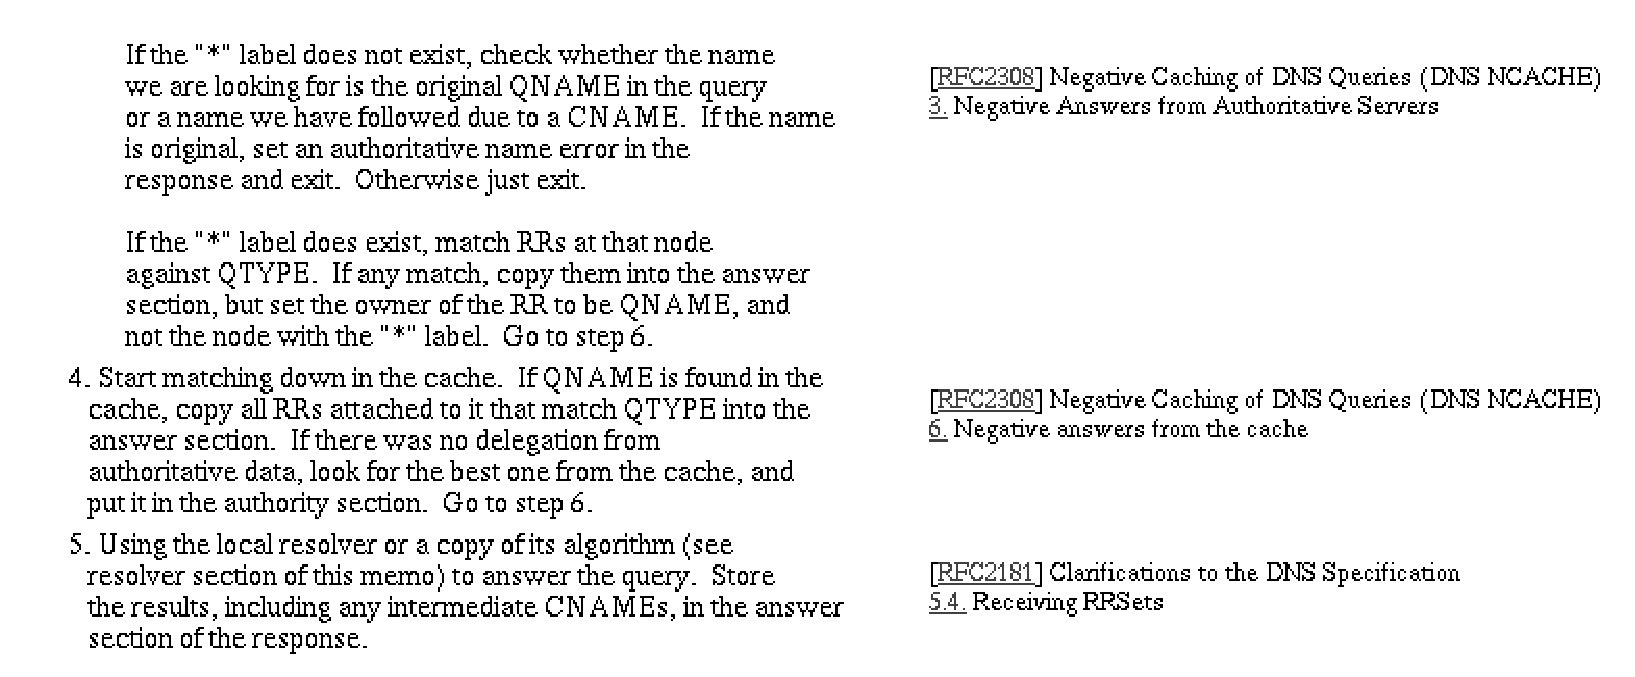
\includegraphics[width=\mockupwidth]{demo4.ps}
%}
%\caption{A mock-up HTML version of a fragment of RFC 1034,
%where the margin contains links to other RFCS that have been
%published later and contain updates relevant to these locations in 
%RFC 1034.
%\label{fig-updatelinks}}
%\end{figure*}

%{\tt title}

%\subsection{subsection1}

%\nakki{tee!}

%----------------------------------------------------------------------------
%\section{RELATED WORK}

%\begin{itemize}
%	\item
%	reflection-in-action process
%	~\cite{nakakoji00spatial-positionin}

%	\item
%	talkback in design
%	~\cite{nakakoji98representational-talkback-in-design}

%	\item
%	bottom-up vs. top-down
%	~\cite{sumi97computer-aided-thinking-and-metric-spaces}
%\end{itemize}

%----------------------------------------------------------------------------
%\section{CONCLUSIONS}

%----------------------------------------------------------------------------
%\section{ACKNOWLEDGMENTS}

% \raggedright

\bibliographystyle{abbrv}
\bibliography{gzigzag}

\end{document}
